\documentclass{article}
\usepackage{graphicx}
\usepackage{tikz}
\usetikzlibrary{arrows,automata}


\begin{document}

\title{Boat Lift}
\author{Filippo Bernardi, Jasper Lustig, Jonas Wallmeier, Snorri Stefansson}

\maketitle

\begin{abstract}
Requirements, description and scope of the project. First meeting.
\end{abstract}

\vspace{3cm}

\begin{figure}[!h]
\centering

	%\path[->, dashed]  (S)  edge              node {a} (l1);
	%\path[->, dotted]  (l1) edge [bend left]  node {a} (S);
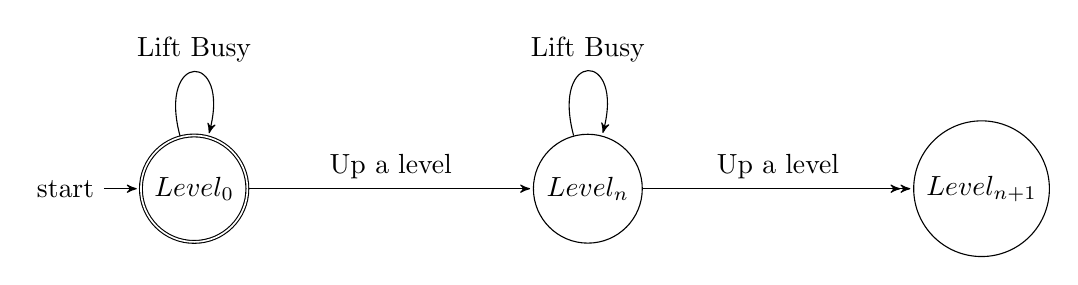
\begin{tikzpicture}[>=stealth',shorten >=1pt,auto,node distance=5cm]
	\node[initial,state,accepting] (S)      {$Level_0$};
	\node[state]         (l1) [right of=S]  {$Level_n$};
	\node[state]         (l2) [right of=l1] {$Level_{n+1}$};
		
	\path  (S)  edge [loop above] node {Lift Busy} (S);
	\path[->]  (S)  edge              node {Up a level} (l1);
	\path  (l1)  edge [loop above] node {Lift Busy} (l1);
	\path[->>] (l1) edge              node {Up a level} (l2);

	edge [bend left]  node {b} (l1);
\end{tikzpicture}
\caption{An extreme simple automata for the boat lift referenced in this document}
\end{figure}

\pagebreak

\section{Introduction}






\section{Conclusion}



\end{document}\grid
